\documentclass{standalone}
\usepackage[dvipsnames]{xcolor}
\usepackage{tikz}
%\usepackage{pgfplots}
%\usepackage{pgfplotstable}
%\pgfplotsset{compat=1.5}
\usetikzlibrary{patterns,decorations.markings}

\begin{document}
{
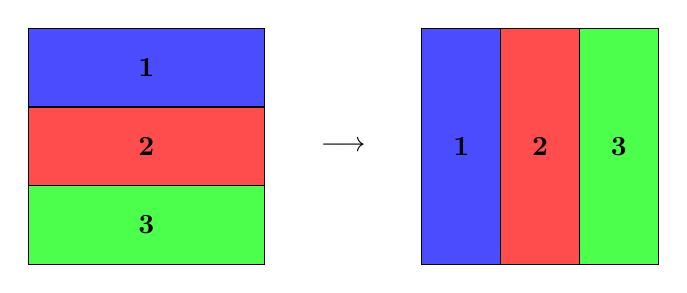
\begin{tikzpicture}
\draw[fill=green!70] (0,0) rectangle (3,1);
\draw[fill=red!70] (0,1) rectangle (3,2);
\draw[fill=blue!70] (0,2) rectangle (3,3);
\node at (1.5,0.5) {\bf 3};
\node at (1.5,1.5) {\bf 2};
\node at (1.5,2.5) {\bf 1};

\begin{scope}[xshift=5 cm]
 \draw[fill=blue!70] (0,0) rectangle (1,3);
\draw[fill=red!70] (1,0) rectangle (2,3);
\draw[fill=green!70] (2,0) rectangle (3,3);
\node at (0.5,1.5) {\bf 1};
\node at (1.5,1.5) {\bf 2};
\node at (2.5,1.5) {\bf 3};
\end{scope}

\node at (4,1.5) {$\longrightarrow$};

\end{tikzpicture}
}
\end{document}